\documentclass[a4paper,12pt]{extarticle}
\usepackage[utf8x]{inputenc}
\usepackage[T1,T2A]{fontenc}
\usepackage[russian]{babel}
\usepackage{hyperref}
\usepackage{indentfirst}
\usepackage{listings}
\usepackage{color}
\usepackage{here}
\usepackage{array}
\usepackage{multirow}
\usepackage{graphicx}
\usepackage{algorithm}
\usepackage{algpseudocode}
\usepackage{caption}
\usepackage{pdfpages}
\usepackage{tikz,mathpazo}
\usepackage{graphicx,amssymb,amstext,amsmath,newtxmath}
\usetikzlibrary{shapes.geometric, arrows}
\renewcommand{\lstlistingname}{Программа} % заголовок листингов кода

\bibliographystyle{ugost2008ls}

\usepackage{listings}
\lstset{ %
extendedchars=\true,
keepspaces=true,
language=C,						% choose the language of the code
basicstyle=\footnotesize,		% the size of the fonts that are used for the code
numbers=left,					% where to put the line-numbers
numberstyle=\footnotesize,		% the size of the fonts that are used for the line-numbers
stepnumber=1,					% the step between two line-numbers. If it is 1 each line will be numbered
numbersep=5pt,					% how far the line-numbers are from the code
backgroundcolor=\color{white},	% choose the background color. You must add \usepackage{color}
showspaces=false				% show spaces adding particular underscores
showstringspaces=false,			% underline spaces within strings
showtabs=false,					% show tabs within strings adding particular underscores
frame=single,           		% adds a frame around the code
tabsize=2,						% sets default tabsize to 2 spaces
captionpos=t,					% sets the caption-position to top
breaklines=true,				% sets automatic line breaking
breakatwhitespace=false,		% sets if automatic breaks should only happen at whitespace
escapeinside={\%*}{*)},			% if you want to add a comment within your code
postbreak=\raisebox{0ex}[0ex][0ex]{\ensuremath{\color{red}\hookrightarrow\space}},
texcl=true,
inputpath=listings,                     % директория с листингами
}

\usepackage[left=2cm,right=2cm,
top=2cm,bottom=2cm,bindingoffset=0cm]{geometry}

%% Нумерация картинок по секциям
\usepackage{chngcntr}
\counterwithin{figure}{section}
\counterwithin{table}{section}

%%Точки нумерации заголовков
\usepackage{titlesec}
\titlelabel{\thetitle.\quad}
\usepackage[dotinlabels]{titletoc}

%% Оформления подписи рисунка
\addto\captionsrussian{\renewcommand{\figurename}{Рисунок}}
\captionsetup[figure]{labelsep = period}

%% Подпись таблицы
\DeclareCaptionFormat{hfillstart}{\hfill#1#2#3\par}
\captionsetup[table]{format=hfillstart,labelsep=newline,justification=centering,skip=-10pt,textfont=bf}

%% Путь к каталогу с рисунками
\graphicspath{{fig/}}

%% Внесение titlepage в учёт счётчика страниц
\makeatletter
\renewenvironment{titlepage} {
 \thispagestyle{empty}
}
\makeatother


\begin{document}	% начало документа

% Титульная страница
\begin{titlepage}	% начало титульной страницы

	\begin{center}		% выравнивание по центру

		\large Санкт-Петербургский политехнический университет Петра Великого\\
		\large Физико-механический институт \\
		\large Высшая школа прикладной математики и вычислительной физики\\[3cm]
		% название института, затем отступ 6см
		\large Направление подготовки\\
		\large "01.03.02. Прикладная математика и информатика"\\[3cm]
		\huge Дисциплина "Численные методы"\\[0.5cm] % название работы, затем отступ 0,5см
		\large Отчет по лабораторной работе №3\\[0.1cm]
		\large "Решение СЛАУ итерационными методами. Метод простых итераций"\\[5cm]

	\end{center}


	\begin{flushright} % выравнивание по правому краю
		\begin{minipage}{0.25\textwidth} % врезка в половину ширины текста
			\begin{flushleft} % выровнять её содержимое по левому краю

				\large\textbf{Работу выполнил:}\\
				\large Иванова А.С.\\
				\large {Группа:} 5030102/00002\\
				
				\large \textbf{Преподаватель:}\\
				\large Курц В.В.

			\end{flushleft}
		\end{minipage}
	\end{flushright}
	
	\vfill % заполнить всё доступное ниже пространство

	\begin{center}
	\large Санкт-Петербург\\
	\large \the\year % вывести дату
	\end{center} % закончить выравнивание по центру

\end{titlepage} % конец титульной страницы

\vfill % заполнить всё доступное ниже пространство


% Содержание
\renewcommand\contentsname{\centerline{Содержание}}
\tableofcontents
\newpage



\section{Формулировка задачи}

Дана функция 
\begin{math} 
	y=\sqrt{\sin{x^{2}}}
\end{math}

График функции:

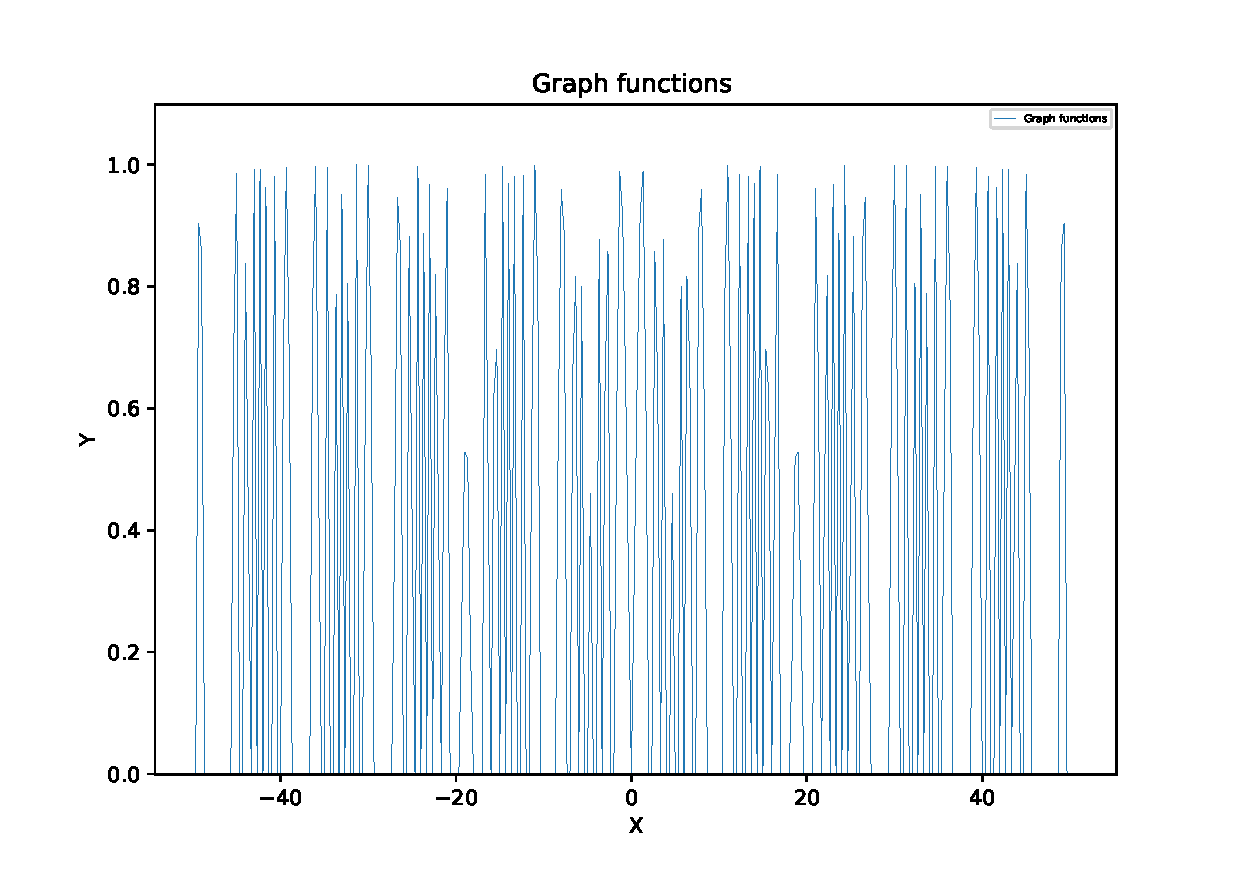
\includegraphics[scale=0.9]{graph.pdf}

Требуется построить интерполяционный полином в форме Лагранжа заданной функции на некотором отрезке [𝑎, 𝑏], используя равномерную сетку и сетку Чебышева. Для этих полиномов исследовать сходимость интерполяционного процесса при разном количестве узлов в сетке, расположении и гладкости функции. 

\section{Алгоритм метода и условия его применимости}

\subsection{Построение сеток}
\subsubsection{Равномерная сетка}
Дан отрезок [a,b], n - количество разбиений. Равномерная сетка 
\begin{math} 
	\{x_{i}\}_{i=0}^{n}
\end{math}
 задается как: 

\begin{math} 
	x_{i}=x_{0}+\frac{(b-a)*i}{n}; i=0,...,n
\end{math}

\subsubsection{Сетка Чебышева}

Дан отрезок [a,b], n - количество разбиений. Сетка Чебышева
\begin{math} 
	\{x_{i}\}_{i=0}^{n}
\end{math}
 задается как: 

\begin{math} 
	x_{i}=\frac{b+a}{2}+\frac{b-a}{2}*\cos{\frac{2i+1}{2(n+1)}*\pi}; i=0,...,n
\end{math}

\subsection{Полином Лагранжа}
Даны некоторая сетка 
\begin{math} 
   \{x_{i}\}_{i=0}^{n}
\end{math}
 и сеточная функция
 \begin{math} 
 	\{y_{i}\}_{i=0}^{n}
 \end{math}. 


Формула полинома Лагранжа: 

 \begin{math} 
	L_{n}(x)=\sum\limits_{i=0}^{n}y_{i}\prod\limits_{k=0 \\* k\neq i}^{n}\frac{x-x_{k}}{x_{i}-x_{k}}
\end{math} 

\subsection{Условия применимости}
Все узлы сетки попарно различны
\section{Предварительный анализ задачи}

При выборе отрезка ненулевой длины для интерполирования получившиеся равномерная сетка и сетка Чебышева могут считаться упорядоченными, а значит все узлы сетки попарно различны. Значит существует интерполяционный полином Лагранжа, и он единственный. 

\section{Проверка условий применимости метода}

При выборе отрезка ненулевой длины для интерполирования получившиеся равномерная сетка и сетка Чебышева могут считаться упорядоченными, а значит все узлы сетки попарно различны. Значит существует интерполяционный полином Лагранжа, и он единственный. 

\section{Тестовый пример с детальными расчетами для задачи малой размерности}

Функция \begin{math} 
	y=\sqrt{\sin{x^{2}}}
\end{math}

Сетка : 
\begin{math} 
	\{-\sqrt{\frac{\pi}{2}};0;\sqrt{\frac{\pi}{2}}\}
\end{math}

Сеточная функция: 
\begin{math} 
	\{1;0;1\}
\end{math}

Полином Лагранжа: 

\begin{math} 
	L(x)=1*\frac{(x-0)(x-\sqrt{\frac{\pi}{2}})}{(-\sqrt{\frac{\pi}{2}}-0)(-\sqrt{\frac{\pi}{2}}-\sqrt{\frac{\pi}{2}})}+0*\frac{(x+\sqrt{\frac{\pi}{2}})(x-\sqrt{\frac{\pi}{2}})}{(0+\sqrt{\frac{\pi}{2}})(0-\sqrt{\frac{\pi}{2}})}+1*\frac{(x+\sqrt{\frac{\pi}{2}})(x-0)}{(\sqrt{\frac{\pi}{2}}+\sqrt{\frac{\pi}{2}})(\sqrt{\frac{\pi}{2}}-0)}=\frac{2x^{2}}{\pi}
\end{math}

\section{Перечень контрольных тестов для иллюстрации метода}

Дана функция 
\begin{math} 
	y=\sqrt{\sin{x^{2}}}
\end{math}

На разных отрезках строился полином Лагранжа для двух типов сеток: равномерной и чебышевской. Степени полинома менялись от 1 до 100 в цикле. Исследуется сходимость интерполяционного процесса (максимальное отклонение полинома от функции от n) на разных участках при разных разбиениях и гладкости функции. 

Данная функция имеет в основном периодическую область определения, разрывов производной на области определения нет, производная не существует на тех участках, где не существует действительных знаечний исходной функции. 

Существует единственный разрыв производной в области опеределения - это точка [0,0]

Рассматривались участки, принадлежащие области определния функции: 

1) [-1.5;1.5], на данном участке присутсвует разрыв производной. 

2) \begin{math} 
	[\sqrt{300*\pi}; \sqrt{301*\pi}]
\end{math}

2) \begin{math} 
	[\sqrt{700*\pi}; \sqrt{701*\pi}]
\end{math}


\section{Модульная структура программы}

def my\_func(x):

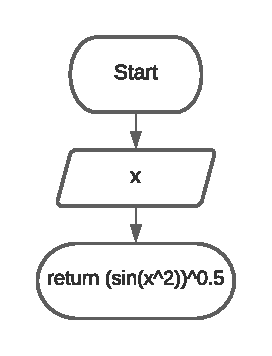
\includegraphics[scale=0.7]{block1.pdf}

def func\_values(func, xlist):

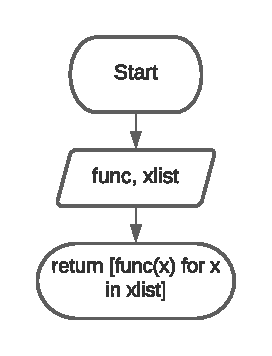
\includegraphics[scale=0.75]{block2.pdf}


def uniform\_grid\_lagrange(x, xmin, xmax, count):

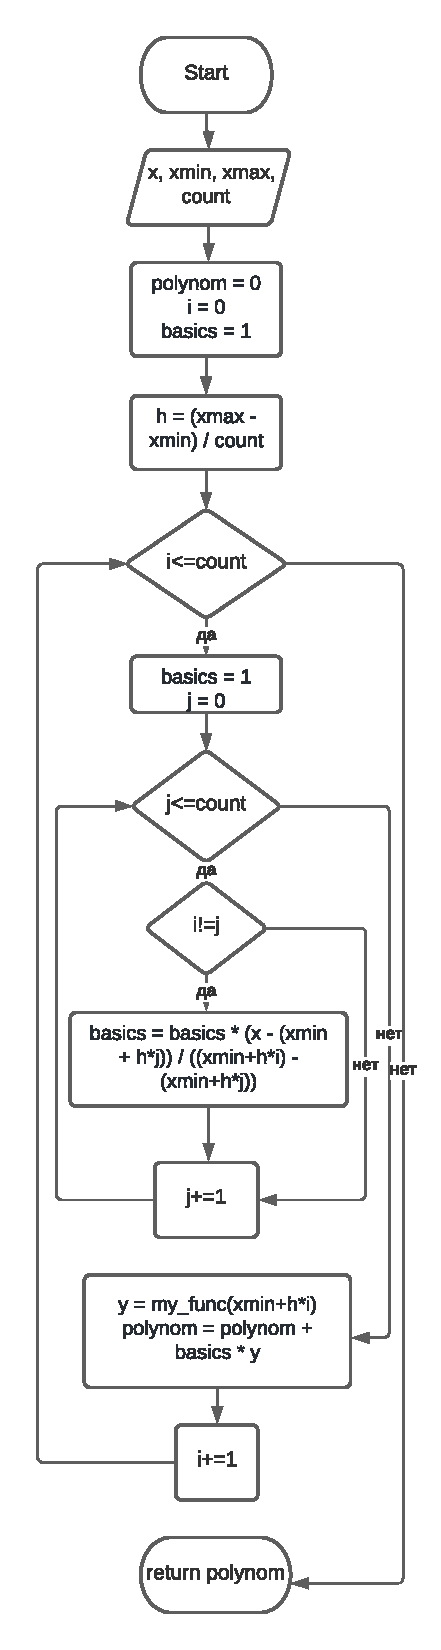
\includegraphics[scale=0.75]{block3.pdf}

\bigskip

def cheb\_grid\_lagrange(x, xmin, xmax, count):

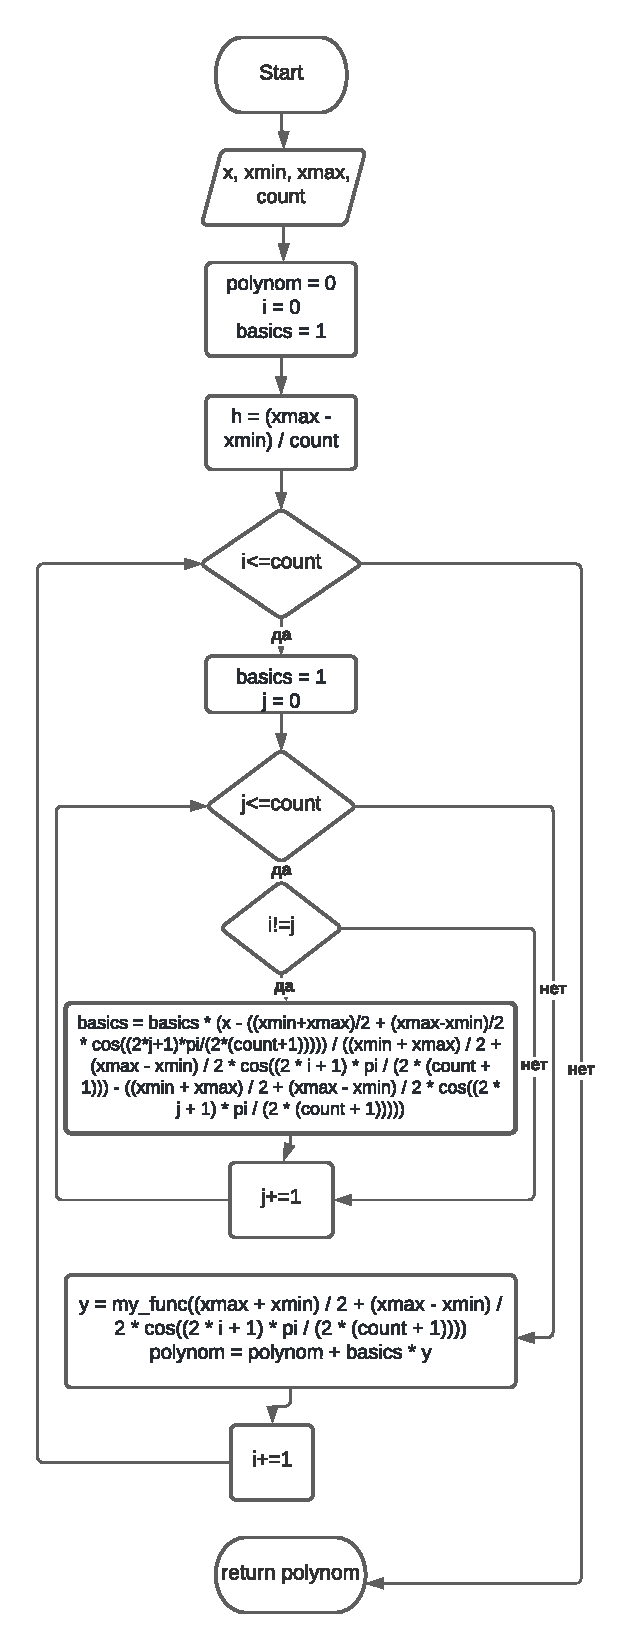
\includegraphics[scale=0.75]{block4.pdf}



\section{Численный анализ решения задачи}

\subsection{\begin{math}[-1.5;1.5]
     \end{math}}

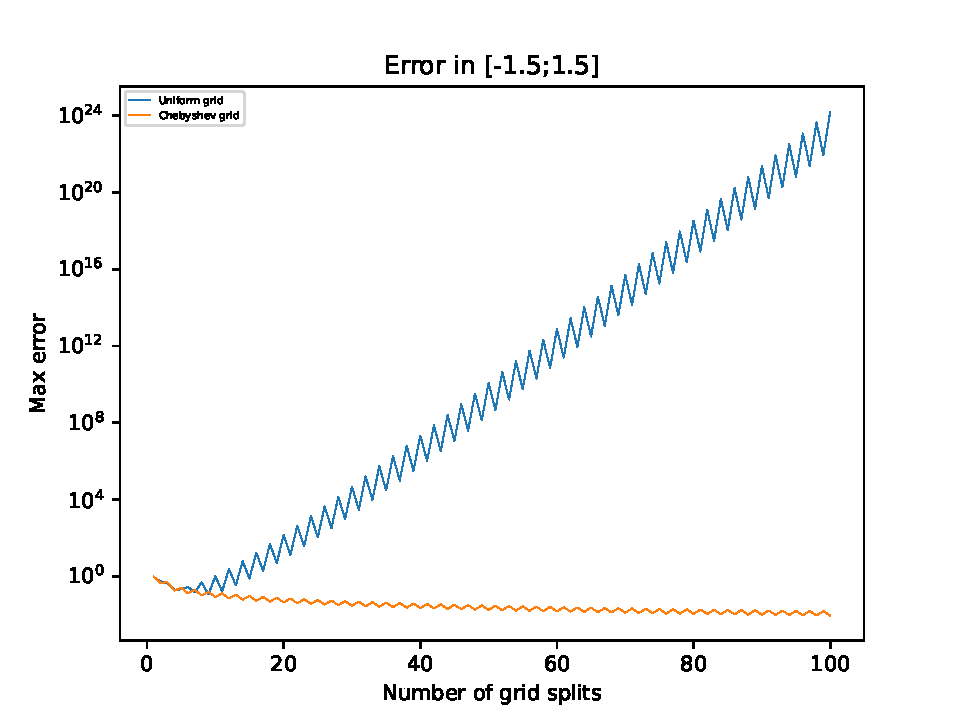
\includegraphics[scale=0.75]{1.pdf}

График зависимости максимального отклонения полинома от функции от количества разбиений. 

Из данного графика видно, что с некоторого значения n при равномерной сетке погрешность начинает сильно возрастать, при использовании сетки Чебышева погрешность постепенно убывает. 

Погрешность для сетки Чебышева убывает очень медленно, а для равномерной сетки очень быстро растет, что обусловлено нарушением гладкости функции. 

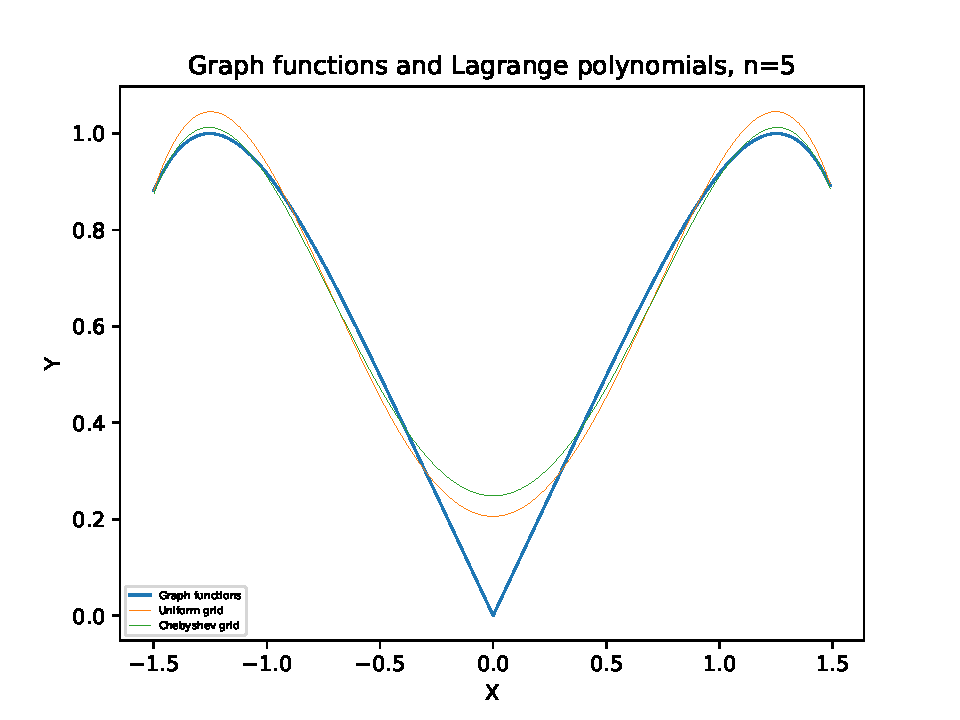
\includegraphics[scale=0.75]{2.pdf}

На данном графике изображены график функции на участке и полиномы Лагранжа для равномерной и чебышевской сетки при n=5. Как видно из графика, поилном с сеткой Чебышева меньше отклоняется от оригинальной функции на гладких участках, но в области разрыва оба полинома дают большую погрешность.

Далее рассматриваются два учатка, входящие в область определния, но не имеющие разрывов производной.

\subsection{ \begin{math} 
		[\sqrt{300*\pi}; \sqrt{301*\pi}]
	\end{math}}

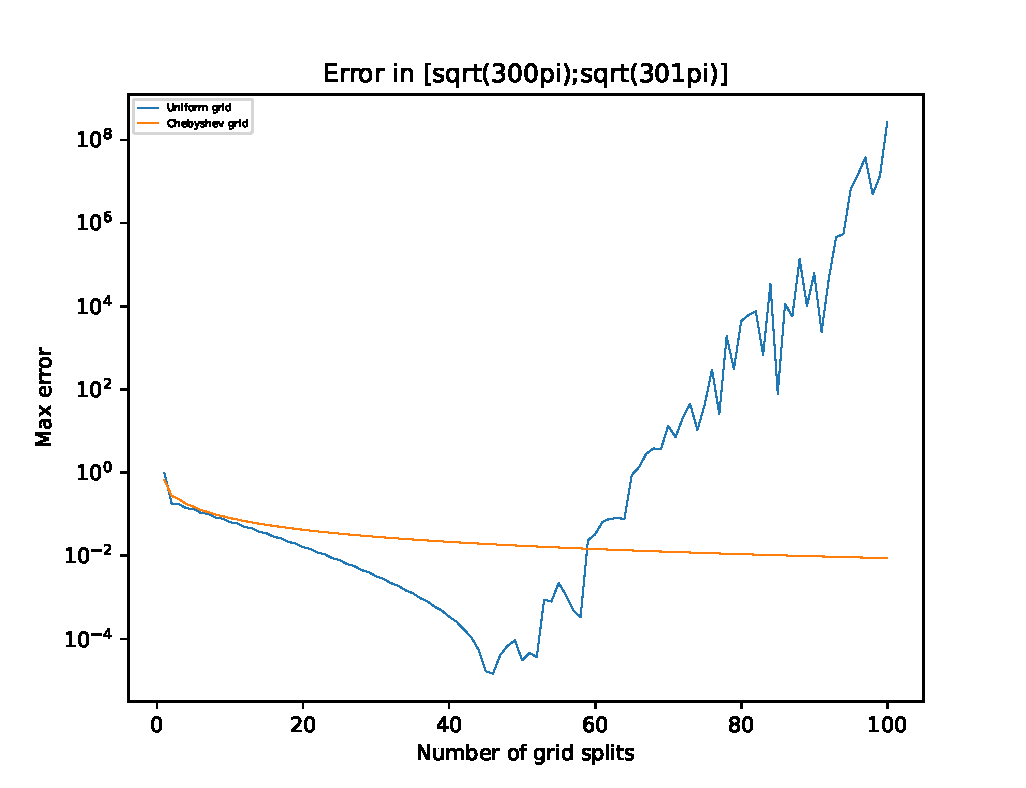
\includegraphics[scale=0.75]{5.pdf}

График зависимости максимального отклонения полинома от функции от количества разбиений. 

Из данного графика видно, что с некоторого значения n при равномерной сетке погрешность начинает сильно возрастать, при использовании сетки Чебышева погрешность постепенно убывает. Но в данном случае погрешность при равномерной сетке возрастает не так сильно, а погрешность при сетке Чебышева убывает сильнее, что связано с отстуствием на данном промежтке разрывов производной.


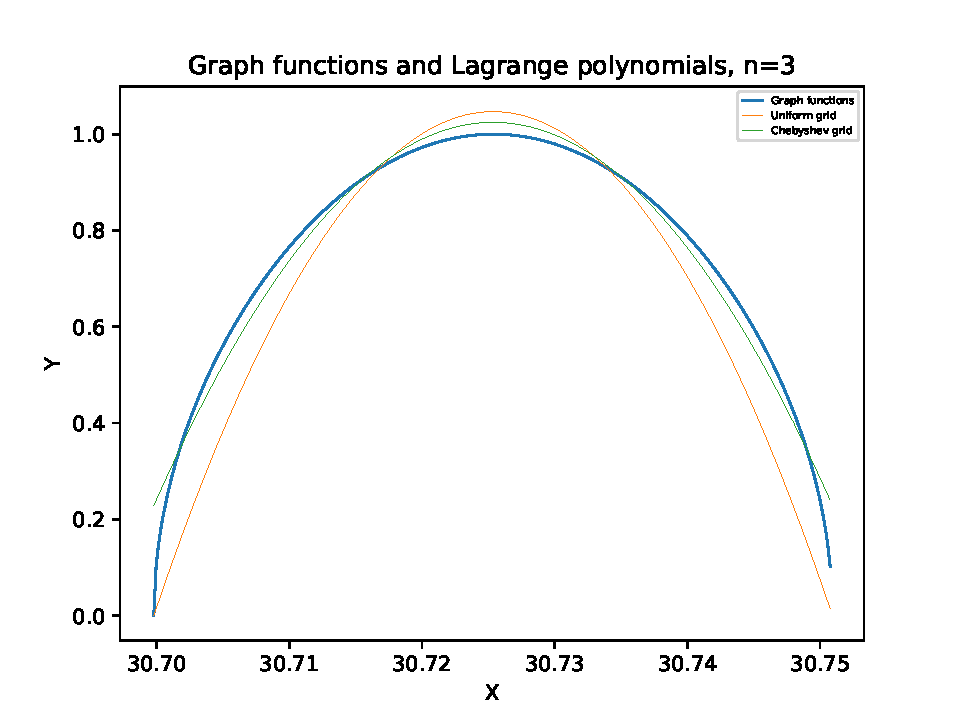
\includegraphics[scale=0.75]{3.pdf}

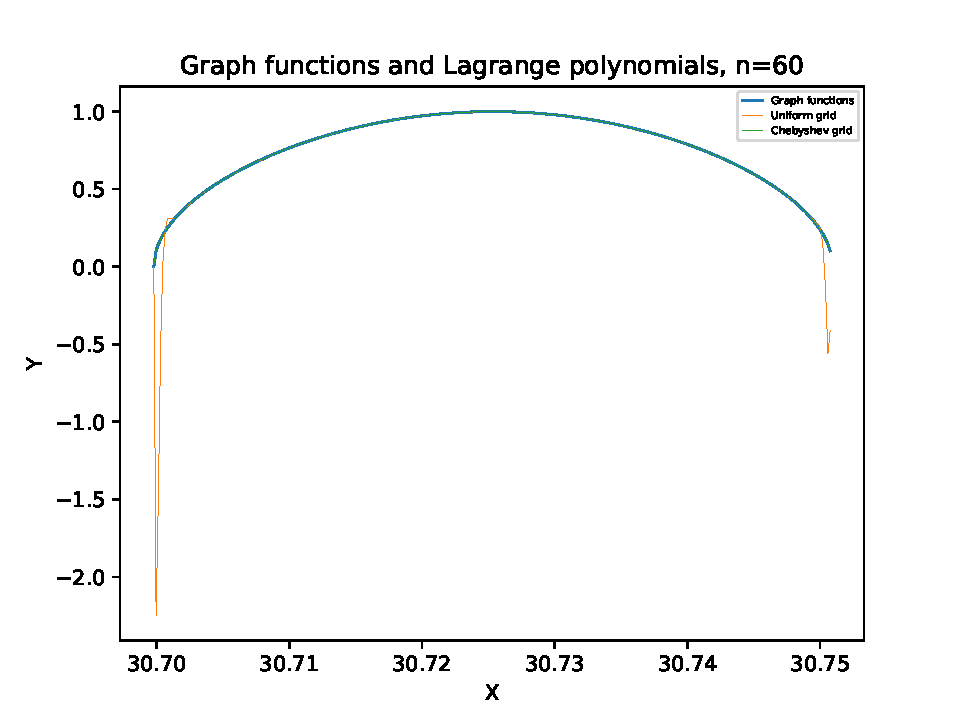
\includegraphics[scale=0.75]{4.pdf}

На данных графиках изображены график функции на участке и полиномы Лагранжа для равномерной и чебышевской сетки при двух различных n. Из первого графика видно, что полином с чебышевской сеткой лучше соответствует графику исходной функции, чем для полинома с равномерной сеткой. А при большом n погрешность становится очень заметной в краевых точках интервала.

\subsection{ \begin{math} 
		[\sqrt{700*\pi}; \sqrt{701*\pi}]
\end{math}}

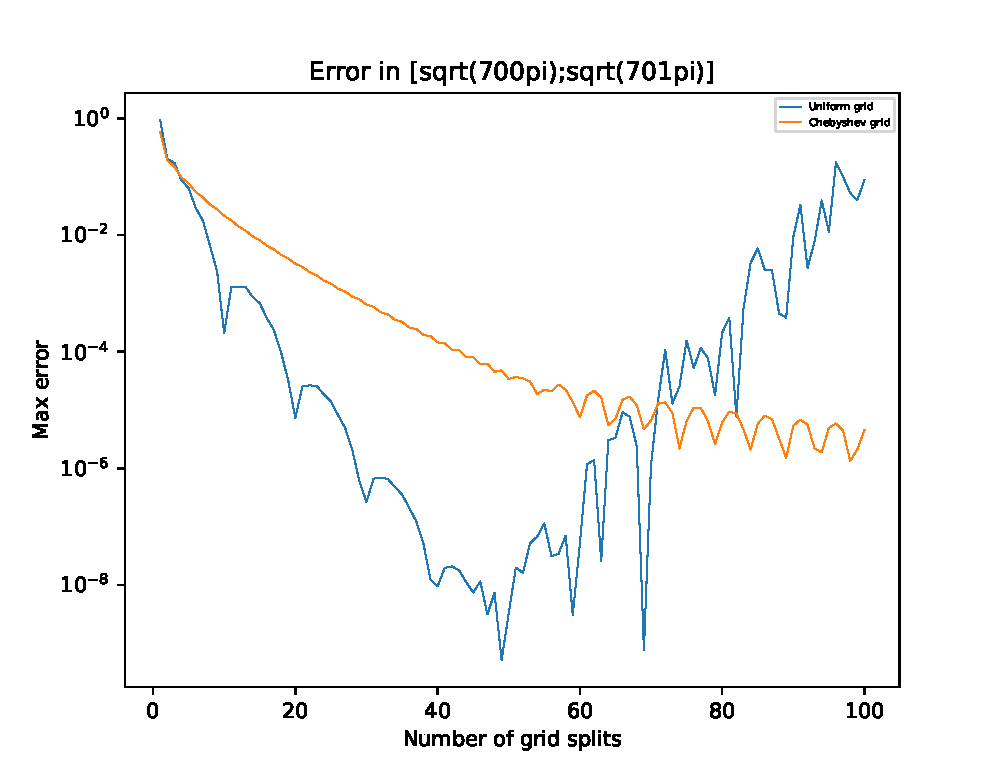
\includegraphics[scale=0.75]{6.pdf}

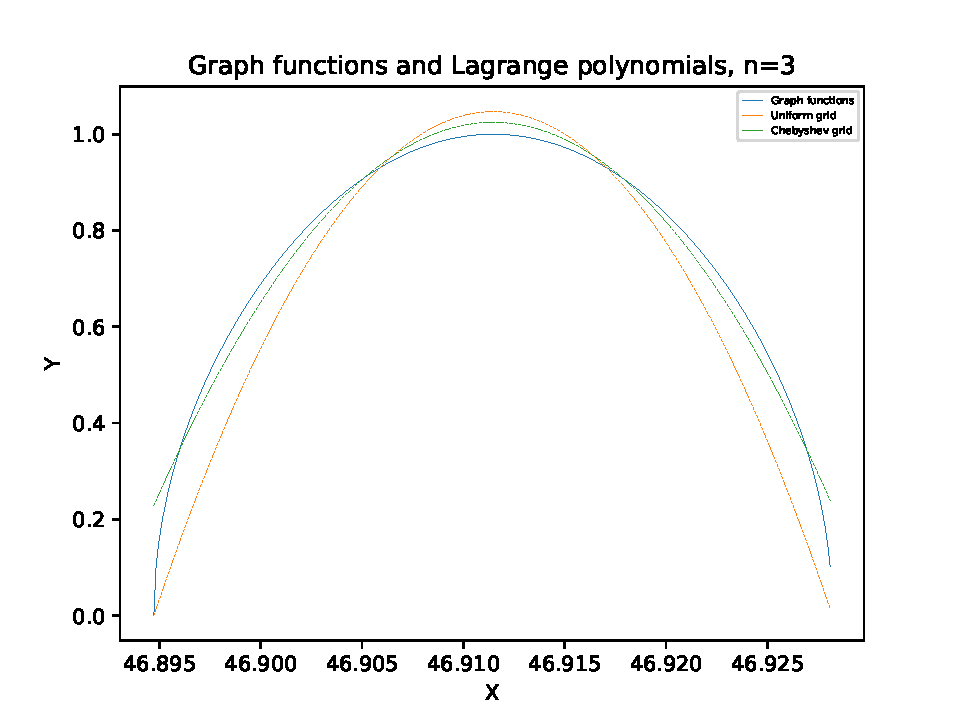
\includegraphics[scale=0.75]{7.pdf}

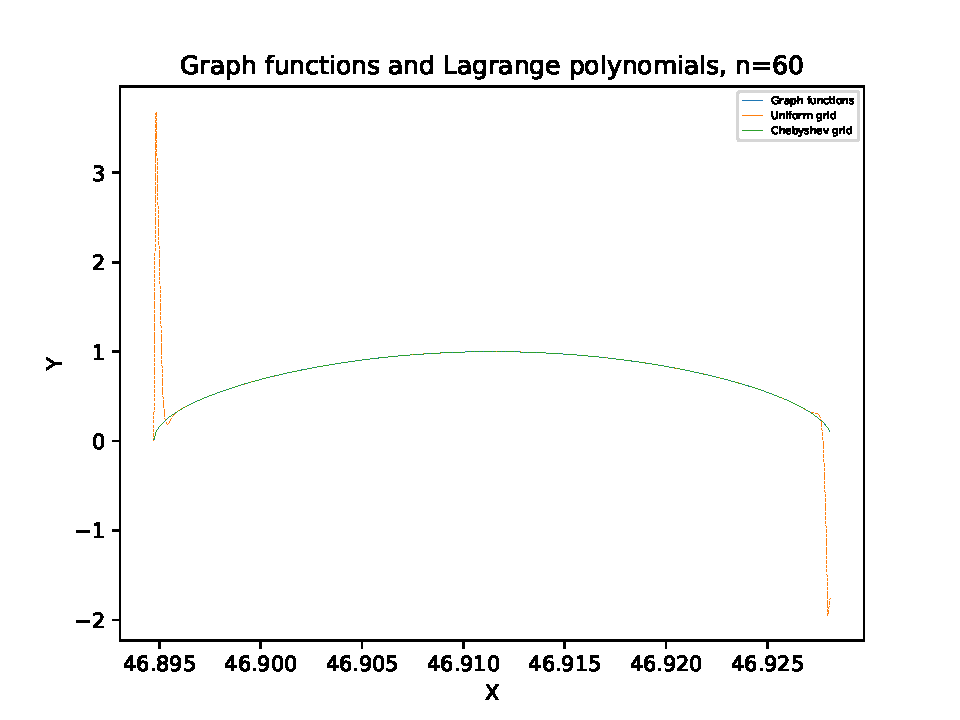
\includegraphics[scale=0.75]{8.pdf}

Да данных графиках сохраняются все ранее полученные результаты для второго интервала, за исключением того, что для равномерной сетки погрешность уменьшается сильнее и при больших n не так быстро возрастает 

\section{Краткие выводы}

На основе полученных результатов можно сделать вывод, что при построении полинома Лагранжа на равномерной сетке при выборе слишком большого числа n (от 40 для гладких участков функции, от 10 для учатсков с разрывом производной) мксимальное отклонение полинома от графика очень сильно возрастает. Данной проблемы можно избежать, если строить полином на сетке Чебышева. 

Гладкость функции также влияет на сходимость интерполяционного процесса. Максимальное отклонение достигает наибольших значений близко к точке разрыва производной, а для равномерной сетки сильно возрастает при увеличении n. 

\end{document}
